This Chapter describes the proposed methodology to implement an image-based gimbal feedback control model for a two-degrees-of-freedom gimbal platform combined with a computer vision system. The solution can be divided into four different stages: Image Acquisition, Object Detection, State Estimation, and Gimbal Control. 

\section{Architecture}
The overall architecture of the proposed system is designed to facilitate real-time object tracking and aiming, integrating several distinct yet interconnected stages. Figure 3.1 illustrates the comprehensive flow of data and the interaction between each primary component, from initial image acquisition to the final aiming mechanism.

The simulated Camera is responsible for capturing a sequence of input image frames, serving as the primary data source for the entire system. The raw image data from the camera is then fed into the Object Detection algorithm.

The Object Detection algorithm processes the incoming image frames to identify and localize the target object. As previously discussed, this module outputs the coordinates of the detected object within each frame. These detected coordinates, though crucial, are prone to noise and inconsistencies.

To address these challenges, the output from the Object Detection stage is passed to the State Estimation module, specifically to the Kalman filter. The Kalman filter plays a vital role by utilizing the noisy coordinate data to estimate the true state of the object, effectively reducing noise, smoothing the signal, and mitigating the effects of data loss or delay. The output of the Kalman filter component is a refined, smoothed trajectory of the target object.

The estimated object state from the Object Tracking module then serves as input for the Motor Controller. This controller translates the object position into a voltage signal for the DC servomotor in the Gimbal Model. The result is an adjustment in the camera's orientation to keep the target object centered in the image. This creates a closed-loop system where the camera's input is processed to control its own orientation, ensuring continuous and accurate tracking of the target object. This integrated architecture ensures a seamless flow from visual input to precise mechanical response, enabling robust object tracking and aiming capabilities.

\begin{figure}[h]
	\centering
	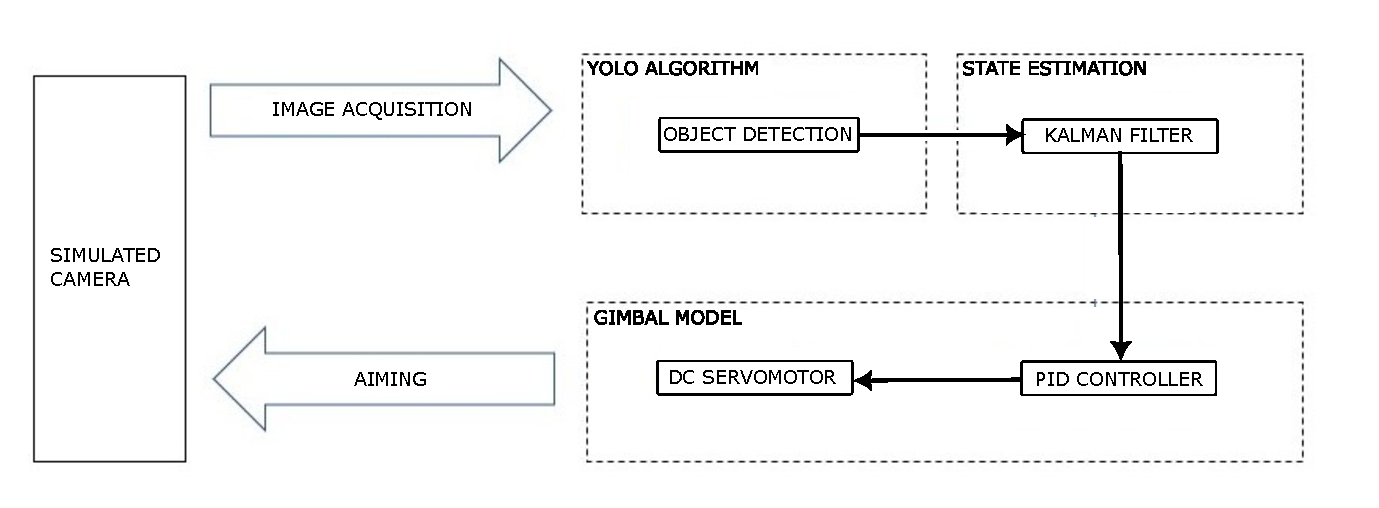
\includegraphics[scale = 0.7]{Cap3/arquitetura.eps}
	\caption{Proposed architecture for the system.}\label{arquiteturaprojeto}
\end{figure}

\section{Image Acquisition}
Images are acquired by a camera coupled in a gimbal, resulting in a configuration similar to the what was presented in Section \ref{secaorefframes}. Every frame captured will serve as input for the object detection algorithm YOLOv8, and the response from the gimbal control will adjust the camera's pointing direction.

A virtual world is created using Simulink\textsuperscript{\textregistered} 3D Animation\textsuperscript{\texttrademark} Toolbox to simulate the camera behavior and image capturing. Further, frames are generated using \textit{Simulation 3D Camera} block. Image \ref{camerasim3d} shows this configuration.

\begin{figure}[H]
	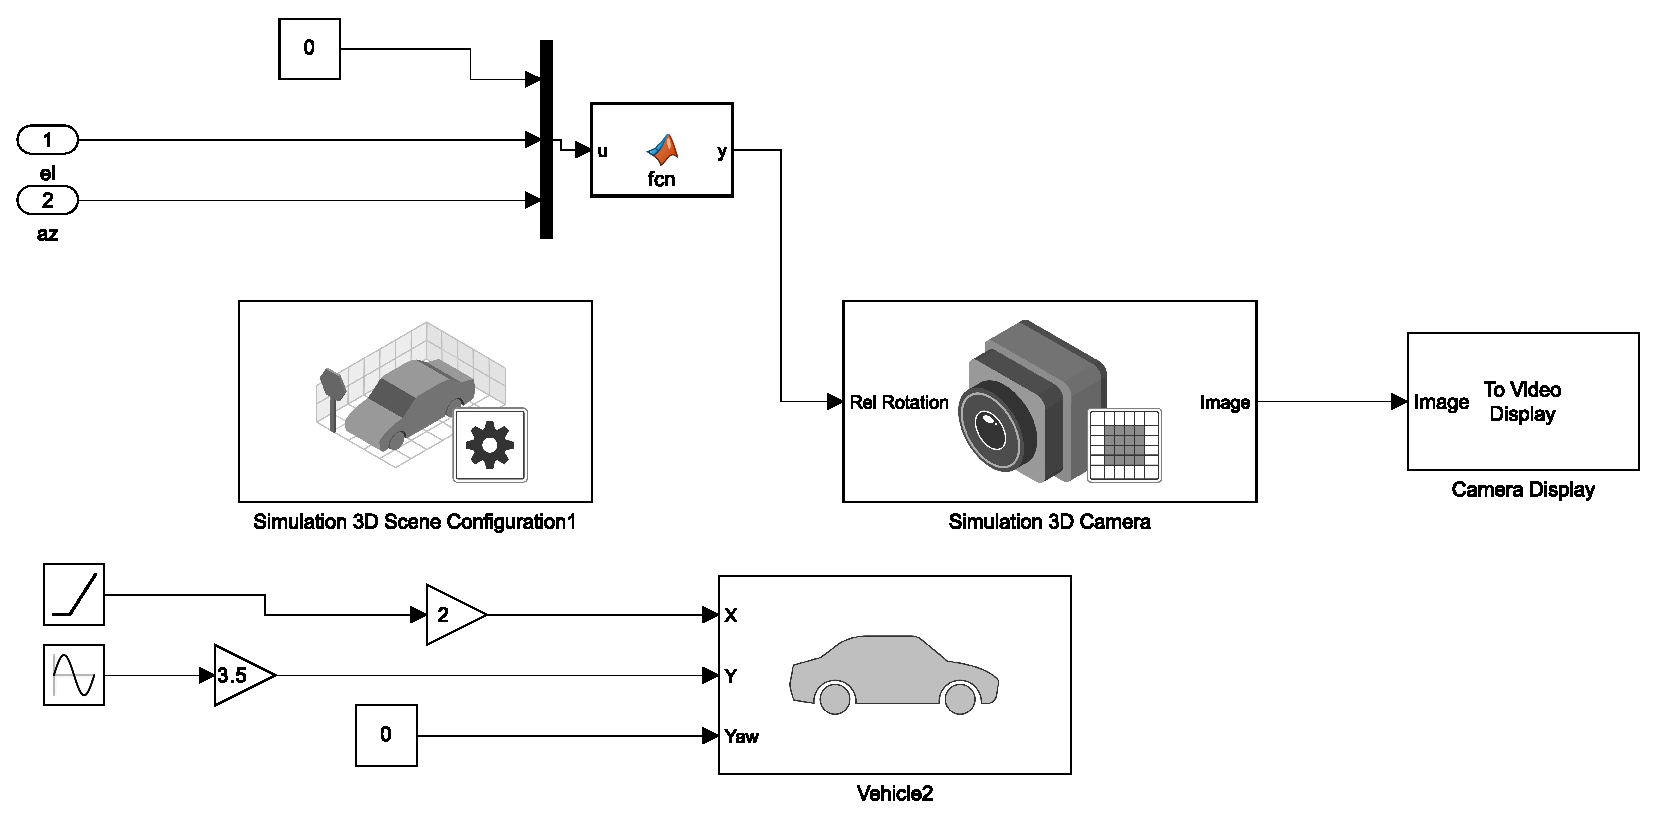
\includegraphics[scale = 0.6]{Cap3/CAMERA_PICTURE.eps}
	\caption{Image acquisition model.}\label{camerasim3d}
\end{figure}

The \textit{Simulation 3D Camera} block maps objects from a three-dimensional space to a two-dimensional space, utilizing the ideal pinhole camera model. The pinhole camera model can be understood as the central projection of points in space onto a plane. According to \citen{Hartley2004}, under the pinhole camera model, a point in space with coordinates $\bm{X} = [X, Y, Z]^T$ is mapped to the point on the image plane where a line joining the point $\bm{X}$ to the centre of projection meets the image plane. Figure \ref{pinholemodel} illustrates this process, with \textbf{C} being the camera centre and \textbf{p} the principal point. The images generated have dimensions of 1280 pixels in width and 720 pixels in height.
\begin{figure}[H]
	\centering
	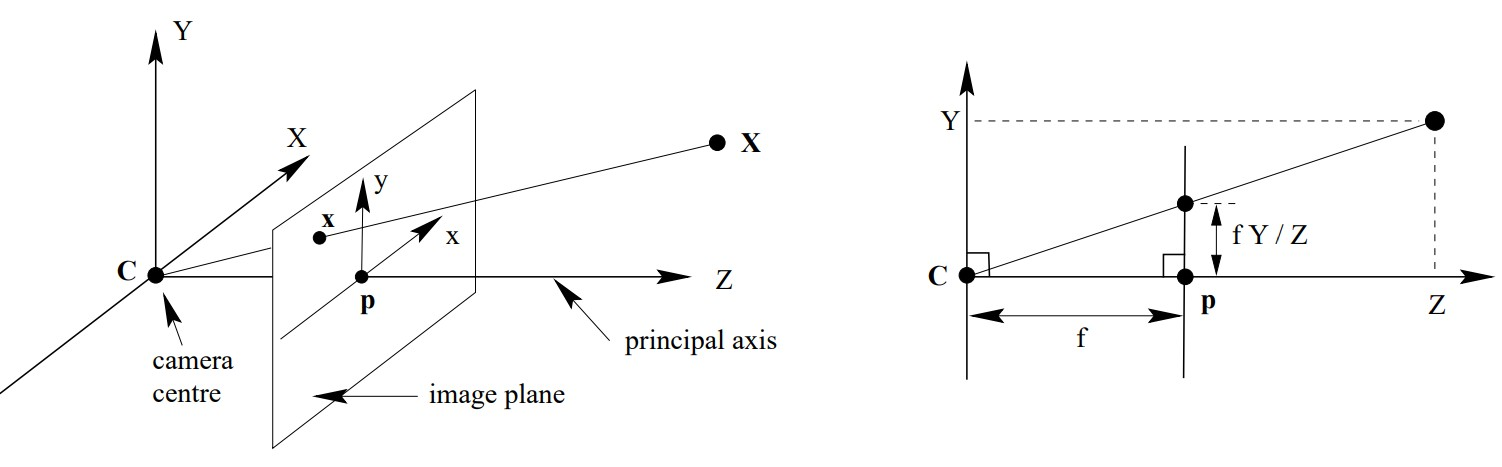
\includegraphics[scale = 0.5]{Cap3/Pinholecamera.jpg}
	\caption{Pinhole camera geometry. Extracted from \citen{Hartley2004}.}\label{pinholemodel}
\end{figure}
The generated frames are displayed in a window using the Camera Display block. The result is shown in Figure \ref{frameresultante}.
\begin{figure}[H]
	\centering
	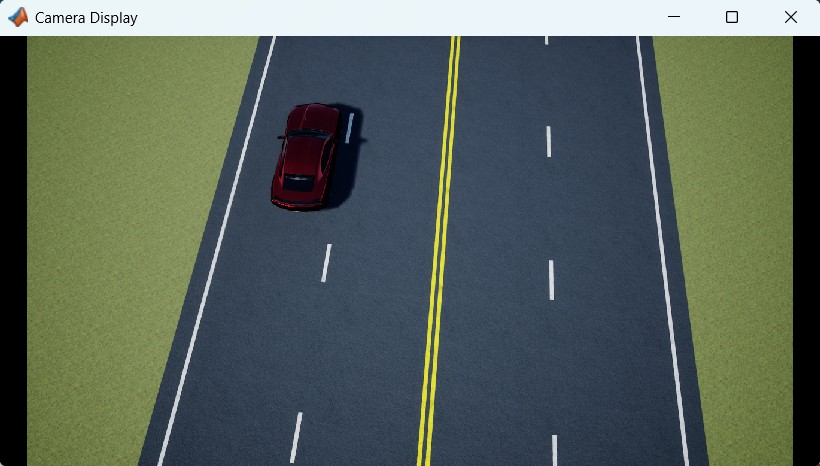
\includegraphics[scale = 0.5]{Cap3/world3d_1.jpg}
	\caption{Resultant frame.}\label{frameresultante}
\end{figure}
With the virtual world and camera correctly modeled, the frames are then recorded using a virtual camera that is generated using the software OBS Studio 31.0.3, which will then be accessed by the object detection algorithm.

\section{Object Detection Algorithm}
The recorded images serve as input to the multi-object detection algorithm YOLOv8, implemented in \textit{Python} programming language using Ultralytics, a computer vision package for object detection and image segmentation models, with a strong focus on the You Only Look Once (YOLO) family of models. The algorithm receives each frame as input and return arrays containing information about the detected object, such as its class, position of the bounding box in the image, and more. We are interested in obtaining the center of the bounding box, represented by a vector $\bm{v} = [x, y]$, where $x$ is the position of the object in the horizontal axis of the image plane in pixels, and $y$ is the position of the object in the vertical axis of the image plane in pixels. Every frame received by YOLOv8 is resized from 1280x720 to 640x480 pixels. Figure \ref{yolografico} shows the pixel range for a given frame.
\begin{figure}[H]
	\centering
	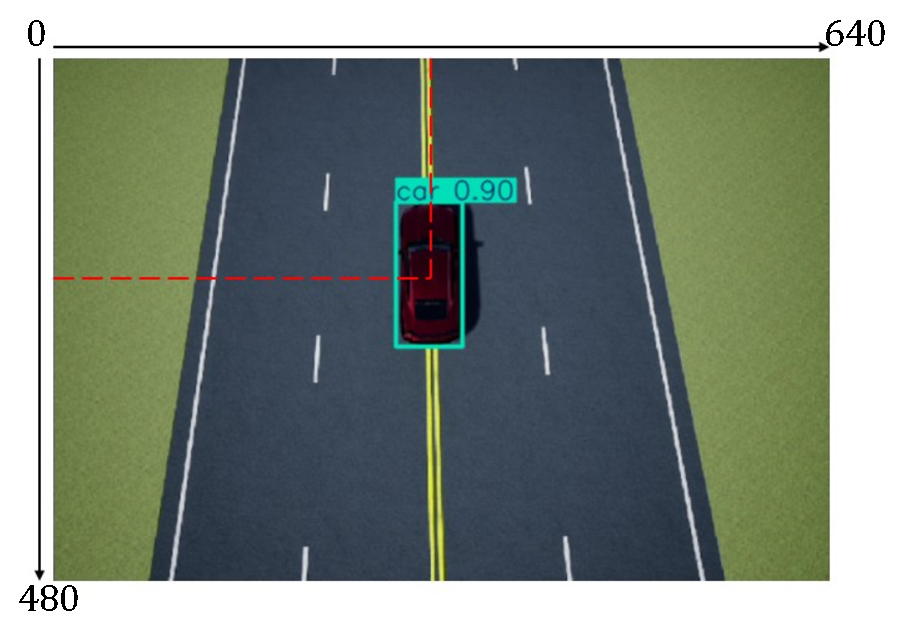
\includegraphics[scale = 0.5]{Cap3/YOLOGRAFICO.eps}
	\caption{Pixel range for each frame.}\label{yolografico}
\end{figure}
This information is then sent to the Simulink model using User Datagram Protocol (UDP) protocol. UDP is a connectionless communication protocol that operates at the transport layer of the Internet Protocol suite. This protocol does not ensure data delivery or order, but ensure low-latency communication, which makes it interesting for data streaming applications \cite{gatimu2020experimental}.

\section{State Estimation}
The object detection algorithm is responsible for recognizing the target object in the input image frame sequence and return its coordinates in every image frame of the acquired sequence. Even though the system is capable of detecting multiple objects, only one object will serve as input for the state estimator algorithm. The raw coordinate data obtained from the object detection algorithm, despite its precision, is inherently susceptible to various forms of noise. This noise can originate from environmental factors, sensor limitations, or even transient occlusions, leading to inconsistencies and abrupt fluctuations in the reported object positions. The Kalman filter is being employed to smooth the received measurements.

The Kalman filter was designed to track a 2D object's position ($x, y$) and velocity ($v_x, v_y$). Its state vector comprises four elements $\hat{\bm{x}} = [x, y, v_x, v_y]^T$. The state transition matrix $A$ models constant velocity, implying that, in the absence of external forces, the object's velocity remains constant, leading to a linear change in its position. However, the inclusion of a non-zero input vector $u$ and the input matrix $B$ further integrates a known, constant acceleration of $[1; 1]$ in both the x and y directions into the model's prediction. The specific matrices are
\begin{equation*}
A = \begin{pmatrix} 1 & 0 & T & 0 \\ 0 & 1 & 0 & T \\ 0 & 0 & 1 & 0 \\ 0 & 0 & 0 & 1 \end{pmatrix}, \quad B = \begin{pmatrix} T^2/2 & 0 \\ 0 & T^2/2 \\ T & 0 \\ 0 & T \end{pmatrix}, \quad u = \begin{pmatrix} 1 \\ 1 \end{pmatrix}.
\end{equation*}

The measurement model is defined by the measurement matrix $C$, which indicates that only the object's 2D position ($x, y$) is directly observed by the sensor (YOLOv8 algorithm). The velocities are not measured, but are estimated by the filter. Thus,
\begin{equation*}
C = \begin{pmatrix} 1 & 0 & 0 & 0 \\ 0 & 1 & 0 & 0 \end{pmatrix}.
\end{equation*}
The time step is set to $T = 0.002$, implying a high sampling rate, which is beneficial for tracking rapidly changing dynamics, but demands a careful scaling of the noise parameters.

The performance of the Kalman filter heavily relies on its noise parameters. The Process Noise Covariance $Q$ matrix accounts for the uncertainty in the object's motion model and any unmodeled accelerations or disturbances. It is derived from $\sigma_{acc} = 2$, making the filter less responsive to changes in velocity, effectively causing it to trust its motion model more, thus ignoring unpredictable movements. The Model Covariance Noise $Q$ is given by
\begin{equation*}
Q = B \cdot M \cdot B^T,
\end{equation*}
where
\begin{equation*}
M = \begin{pmatrix} \sigma_{acc}^2 & 0 \\ 0 & \sigma_{acc}^2 \end{pmatrix}.
\end{equation*}
Conversely, the Measurement Noise Covariance $R$ matrix represents the expected noise in the incoming YOLOv8 position measurements. The standard deviation $\sigma_{cam} = 1000$ indicates that the filter considers the input signal to be extremely noisy. This high $\sigma_{cam}$ value means the filter will place very little weight on the instantaneous YOLOv8 measurements, instead relying heavily on its internal predictions and previous estimates to produce a smooth output. Measurement Noise Covariance matrix $R$ is writen as

\begin{equation*}
R = \begin{pmatrix} \sigma_{cam}^2 & 0 \\ 0 & \sigma_{cam}^2 \end{pmatrix}.
\end{equation*}

Using the methodology proposed in Section \ref{secaokalmanfilter} associated with the described model, the result for the filtering process is given by Table \ref{kalmanfilterprocess}.

\begin{table}[H]
\begin{center}
\caption{Resultant equations for the Kalman filter recursive process.}
\label{kalmanfilterprocess}
\begin{tabular}{|c||c|} 
 \hline
 Description & Equation \\ [0.5ex] 
 \hline\hline
 Kalman Gain & $K_k = P'_kC^T(CP'_kC^T + R)^{-1}$\\ 
 \hline
 Update Estimate & $\hat{\bm{x}}_k = \hat{\bm{x}}'_k + K_k(z_k - C\hat{\bm{x}}'_k)$\\
 \hline
 Update Covariance & $P_k = P'_k - K_k C P'_k$\\
 \hline
 Project into $k+1$ & $\hat{\bm{x}}_{k+1} = A \hat{\bm{x}}_k$ \\
					& $P_{k+1} = A P_k A^T + Q$ \\
 \hline
\end{tabular}
\end{center}
\end{table}

Figure \ref{kalmanfiltergrafico} shows the comparison between the received signal from YOLOv8 and the output from the Kalman filter.
\begin{figure}[H]
	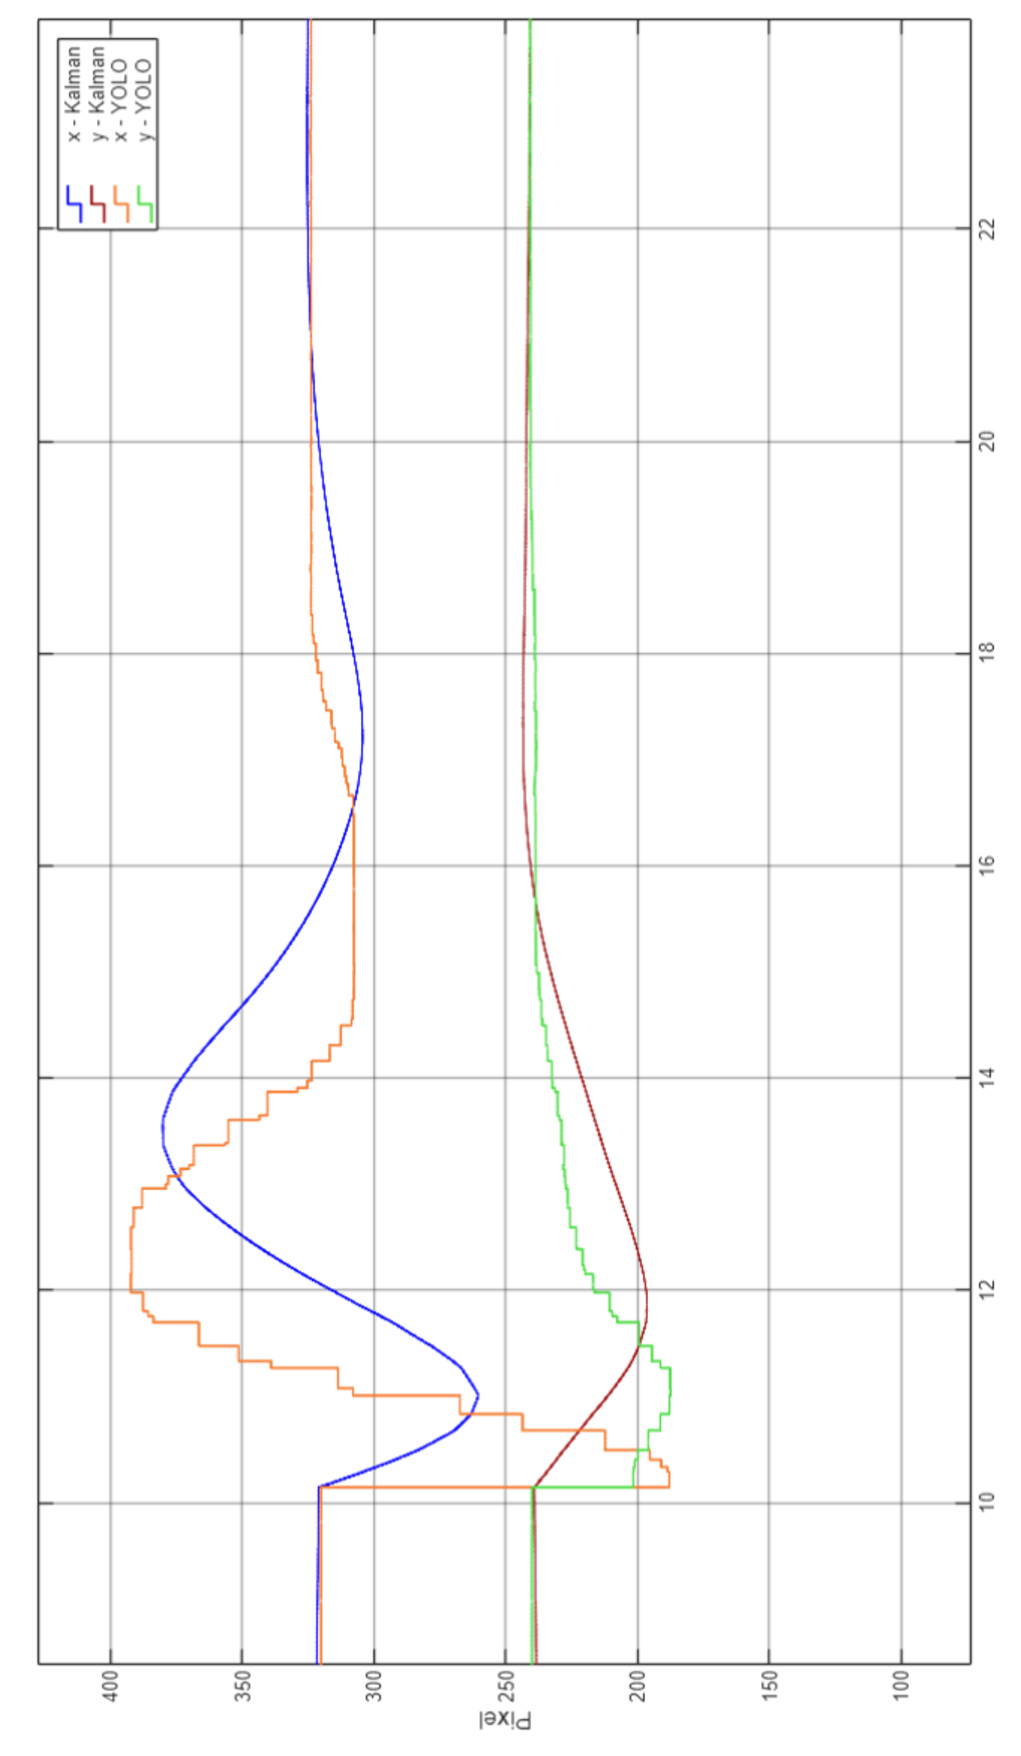
\includegraphics[scale = 0.54, angle = 270]{Cap3/kalmanfilter.eps}
	\caption{Kalman filter applied to the YOLOv8's detections.}\label{kalmanfiltergrafico}
\end{figure}

\subsection{Post Filter Processing}
After the Kalman filter, a processing step is responsible for preparing the signal for the controller. The purpose is to shape the signal according to the camera's field-of-view. Firstly, a gain is applied to rescale the signal to 1280x720 pixels, matching the simulated camera's output dimensions. Then, using the camera's intrinsic matrix associated with homogeneous coordinates, we normalize the received vector and translate the information to angular position. 
The first step is to convert the raw 2D pixel coordinates ($u,v$) from the image plane into normalized image coordinates ($x_n,y_n$) in the camera's coordinate system. This process effectively inverts the camera's intrinsic matrix (focal length, principal point), as represented in equation \ref{intrinsic matrix}. 
\begin{equation}
	\label{intrinsic matrix}
     \left[\begin{matrix}x_c \\ y_c \\ z_c\end{matrix}\right] = K^{-1}\left[\begin{matrix}u \\ v \\ 1 \end{matrix}\right].
\end{equation}
The intrinsic matrix \cite{Hartley2004} is represented as
\begin{equation}
	\label{intrmatri}
    K = \left[\begin{matrix} f_x & 0 & c_x \\0 & f_y & c_y\\ 0 & 0 & 1\end{matrix}\right],
\end{equation}
where $f_x$ and $f_y$ represents the focal length in x and y directions, respectively, and $c_x$ and $c_y$ represent the coordinates of the principal point. With the normalized vector, a gain is applied to generate a signal that represents the object's position with relation to the camera's field-of-view for each axis, in radians.

\section{Gimbal Model}
The dynamics of the two-degrees-of-freedom gimbal is modeled using Simulink, and the communication with the object detection algorithm will result in the system's response to the input images, ensuring that the camera is pointing to the desired target. The model is reduced to the elevation and azimuth axes, where in each case the respective inertia is represented. For each axis, there is a controlled electrical motor responsible for the torque that rotates the mass. The model is implemented via transfer function. 

\subsection{Rotational Axes}
\label{secaorotationalaxes}
The rotational axes are divided into 3 main blocks: the Controller, the DC motor and the Gimbal (for elevation and azimuth). Starting with the Inner Gimbal, the rotational movement expressed in equation \eqref{Momento angular y inner 1} is used. Given that the only source of torque is the electrical motor, the equation can be rewriten as
\begin{equation}
   \label{Momento angular y inner 1}
   T_{m_I} = I^I_y \alpha_{IB_y} + (I^I_x - I^I_z) \Omega_{IB_x} \Omega_{IB_z} + T_{\text{Friction}_{OI}}.
\end{equation}
This express the torque needed from the motor to rotate the mass. As mentioned in Section \ref{secaodinamicagimbal}, some considerations are adopted to simplify the model. By eliminating the effects from Cross-Coupling, the equation is now
\begin{equation}
   T_{m_I} = I^I_y \alpha_{IB_y} + T_{\text{Friction}_{OI}}.
\end{equation}
The Coulomb friction model is an distrubance in the torque signal due to the non linear nature of this phenomenon. Therefore, the final equation for the inner gimbal rotational dynamic becomes a linear function expressed as
\begin{equation}
   \label{Momento angular y inner reduced}
   T_{m_I} = I^I_y \alpha_{IB_y} + k_{vf}\Omega_{IB_y}.
\end{equation}
The same process is applied to the outer gimbal, resulting in the equation
\begin{equation}
	\label{momento angular z outer}
T_{m_O} = I^O_z \alpha_{{OB}_z} + k_{vf}\Omega_{OB_z}.
\end{equation}
Table \ref{tabelaparametrogimbal}, extracted from \citen{espinosa2016diseno} shows the inertial parameters for the inner and outer gimbals.
\begin{table}[H]
\begin{center}
\caption{Gimbal's Inertial Parameters.}
\label{tabelaparametrogimbal}
\begin{tabular}{|c||c|} 
 \hline
 Parameter & Value \\ [0.5ex] 
 \hline\hline
 $I^I_x$ & $1.68 \times 10^{-4} \, (\text{kg} \cdot \text{m}^2)$\\ 
 \hline
 $I^I_y$ & $1.78 \times 10^{-4} \, (\text{kg} \cdot \text{m}^2)$ \\
 \hline
 $I^I_z$ & $1.16 \times 10^{-4} \, (\text{kg} \cdot \text{m}^2)$ \\
 \hline
 $I^O_x$ & $2.62 \times 10^{-3} \, (\text{kg} \cdot \text{m}^2)$ \\
 \hline
 $I^O_y$ & $2.47 \times 10^{-3} \, (\text{kg} \cdot \text{m}^2)$ \\
 \hline
 $I^O_z$ & $4.66 \times 10^{-4} \, (\text{kg} \cdot \text{m}^2)$ \\
 \hline
\end{tabular}
\end{center}
\end{table}

\subsection{Electrical Motors}
\label{secaoelectricalmotors}
The electrical motors are the source of torque in both axes, azimuth and elevation. These motors will be responsible for converting the voltage signal into a torque, and are modeled using the equivalent circuit diagram of DC servo motors, as shown in figure \ref{servomotor}.
\begin{figure}[H]
	\centering
	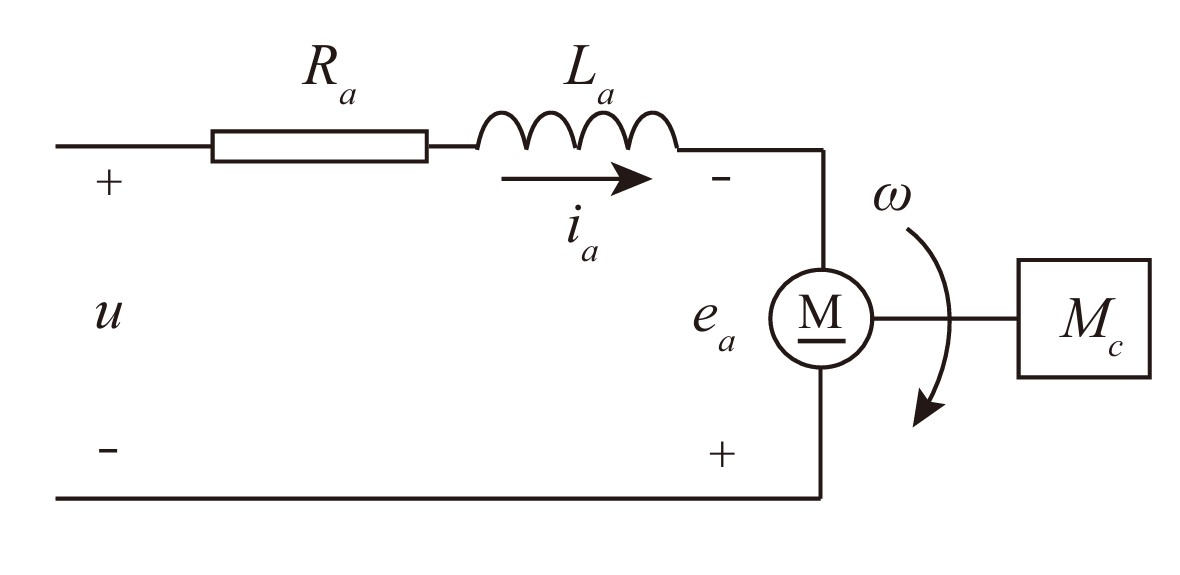
\includegraphics[scale = 0.4]{Cap3/Servomotorcircuit.jpg}
	\caption{Equivalent circuit diagram of DC servo motor. Extracted from \citen{servomotorarticle}.}\label{servomotor}
\end{figure}
In this representation, $R_a$ is the resistance of the armature coil, $L_a$ is the armature inductance, $i_a$ is the armature current, $e_a$ is the counter electromotive force, $u$ is the applied voltage, $\omega$ ($\Omega$ in our system) is the rotational speed, and $M_c$ is the load torque. Using Kirchhoff's Voltage law, this circuit can be mathematically expressed as
\begin{equation}
	\label{equacao do servo motor}
	u(t) = R_a i_a(t) + L_a \dot i_a(t) + e_a(t).  
\end{equation}

The counter electromotive force is the relation between the counter electromotive constant, $K_e$, and the rotational speed, that is the first derivative of the angular position in relation to time, $\dot \theta(t)$. This allows us to rewrite equation \eqref{equacao do servo motor} into
\begin{equation}
	\label{equacaout}
	u(t) = R_a i_a(t) + L_a \dot i_a(t) + K_e \dot \theta(t).  
\end{equation}
Lastly, the equation for the load torque is given as follows:
\begin{equation}
	\label{equacaoMC}
	M_c(t) = C_m i_a(t),
\end{equation}
where $C_m$ is the torque constant and $i_a(t)$ is the armature current. The electrical motors are modeled using the parameters of the FAULHABER\textsuperscript{\textregistered} 1524T012SR DC motor (Figure \ref{FAULHABERMOTOR}). Table \ref{tabelaparametromotor} shows the parameters for this DC motor.
\begin{figure}[H]
	\centering
	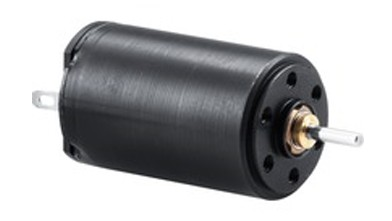
\includegraphics[scale = 0.5]{Cap3/FAULHABER.jpg}
	\caption{FAULHABER\textsuperscript{\textregistered} 1524T012SR.}\label{FAULHABERMOTOR}
\end{figure}

\begin{table}[H]
\begin{center}
\caption{FAULHABER\textsuperscript{\textregistered} 1524T012SR parameters}
\label{tabelaparametromotor}
\begin{tabular}{|c||c|}
\hline
Parameter & Value \\ [0.5ex]
\hline\hline
Nominal Voltage & 12 [V] \\
\hline
Armature resistance & 0.674 [$\Omega$] \\
\hline
Output Power & 1.75 [W] \\
\hline
Max efficiency & 0.76 \\
\hline
No-load speed & 9900 [rpm] \\
\hline
No-load current & 0.011 [A] \\
\hline
Friction torque & 0.13 [mNm] \\
\hline
Speed constant & 840 [rpm/V] \\
\hline
Torque constant & 11.4 [mNm/A] \\
\hline
Armature Inductance & 250 [$\mu$H] \\
\hline
Rotor inertia & 0.65 [g cm\textsuperscript{2}] \\
\hline
Angular acceleration & 100$\times 10^3$ [rad/s\textsuperscript{2}] \\
\hline
Weight & 21 [g] \\
\hline
Stall torque & 6.92 10\textsuperscript{-3} [Nm] \\
\hline
\end{tabular}
\end{center}
\end{table}
Associated with the electrical motor, the parameters of the encoder are given in Table \ref{tabela encoder}. Encoders are vital components in DC servomotor systems, providing crucial feedback for precise control of position, speed, and direction. They essentially translate the motor's rotational motion into electrical signals that a controller can interpret. In this work, the parameters of FAULHABER\textsuperscript{\textregistered} IE2-512 are being used.
\begin{table}[H]
\begin{center}
\caption{FAULHABER\textsuperscript{\textregistered} IE2-512 parameters.}
\label{tabela encoder}
\begin{tabular}{|c||c|} 
 \hline
 Parameter & Value \\ [0.5ex] 
 \hline\hline
 Pulses per resoluton & 512\\ 
 \hline
 Max frequency & 160$\times$10\textsuperscript{3} [Hz]\\
 \hline
 Inertia & 0.09 [g·cm²]\\
 \hline
 Phase shift & 90 [$^\circ$]\\
 \hline
\end{tabular}
\end{center}
\end{table}

\subsection{Transfer Functions}
Using equations \eqref{Momento angular y inner reduced}, \eqref{equacaout} and \eqref{equacaoMC}, the transfer function that relates input voltage to motor torque ($T_{m_I}(s)/U(s)$) and motor torque to angular position ($\Theta (s)/T_{m_I}(s)$) can be obtained. To give more realism to these functions, the viscous friction is augmented with the motor's bearings friction and the rotational inertia of the motor and encoder are also considered. Thus, assuming zero initial conditions, the Laplace transform of these equations yields:
\begin{itemize}
\item From \eqref{Momento angular y inner reduced}:
\begin{equation*}
    T_{m_I}(s) = I_y^I s^2 \Theta(s) + k_{vf} s \Theta(s)
\end{equation*}
\begin{equation}
	\label{3.8}
    T_{m_I}(s) = (I_y^I s + k_{vf}) s \Theta(s)
\end{equation}
\item From \eqref{equacaout}:
\begin{equation*}
    U(s) = R_a I_a(s) + L_a s I_a(s) + K_e s \Theta(s)
\end{equation*}
\begin{equation}
	\label{equacaodomotordclaplace}
    U(s) = (R_a + L_a s)I_a(s) + K_e s \Theta(s)
\end{equation}
\item From \eqref{equacaoMC}:
\begin{equation}
	\label{3.10}
    T_{m_I}(s) = C_m I_a(s)
\end{equation}
\end{itemize}

To derive $\frac{T_{m_I}(s)}{U(s)}$, we first express $I_a(s)$ and $s\Theta(s)$ in terms of $T_{m_I}(s)$ using equations \eqref{3.10} and \eqref{3.8}:
\begin{equation}
	\label{3.11}
I_a(s) = \frac{T_{m_I}(s)}{C_m}
\end{equation}
\begin{equation}
	\label{3.12}
s\Theta(s) = \frac{T_{m_I}(s)}{I_y^I s + k_{vf}}
\end{equation}
Now, by using \eqref{3.11} and \eqref{3.12} into \eqref{equacaodomotordclaplace} (in Laplace domain):
$$U(s) = (R_a + L_a s) \left(\frac{T_{m_I}(s)}{C_m}\right) + K_e \left(\frac{T_{m_I}(s)}{I_y^I s + k_{vf}}\right)$$
Factoring $T_{m_I}(s)$ from the right-hand side:
$$U(s) = T_{m_I}(s) \left[ \frac{R_a + L_a s}{C_m} + \frac{K_e}{I_y^I s + k_{vf}} \right]$$
Applying algebraic manipulations, we can obtain the desired transfer function
\begin{equation}
\frac{T_{m_I}(s)}{U(s)} = \frac{C_m (I_y^I s + k_{vf})}{L_a I_y^I s^2 + (R_a I_y^I + L_a k_{vf})s + (R_a k_{vf} + C_m K_e)},
\end{equation}
where $T_{m_I}(s)$ represents the Laplace transform of the motor torque, $U(s)$ denotes the Laplace transform of the input voltage to the motor, and $I_y^I$ is the moment of inertia of the inner gimbal about its y-axis. The viscous friction coefficient is denoted by $k_{vf}$, while $R_a$ and $L_a$ represent the armature resistance and armature inductance of the motor, respectively. $C_m$ is the motor torque constant, $K_e$ is the back-EMF constant, and $s$ is the Laplace operator.

The transfer function from motor torque to angular position ($\Theta (s)/T_{m_I}(s)$) is directly obtained from equation \eqref{Momento angular y inner reduced}:
\begin{equation}
    \frac{\Theta(s)}{T_{m_I}(s)} = \frac{1}{(I_y^I s + k_{vf}) s}
\end{equation}

Similarly, the transfer functions for the outer gimbal are obtained:
\begin{equation}
\frac{T_{m_O}(s)}{U(s)} = \frac{C_m (I_z^O s + k_{vf})}{L_a I_z^O s^2 + (R_a I_z^O + L_a k_{vf})s + (R_a k_{vf} + C_m K_e)},
\end{equation}
\begin{equation}
    \frac{\Theta(s)}{T_{m_O}(s)} = \frac{1}{(I_z^O s + k_{vf}) s}
\end{equation}

Figure \ref{fig:modelototal} illustrates the implementation in Simulink.

\begin{figure}[H]
    \centering
    \begin{tabular}{c} % 'c' for centered content in a single column
        
\includegraphics[scale = 0.5, angle = 270]{cap3/inomeado.eps} \\ % Replace image1.png with your first image file
        
\includegraphics[scale = 0.5, angle = 270]{cap3/DCmotorouter.eps} % Replace image2.png with your second image file
    \end{tabular}
    \caption{Simulink model for DC servomotor and gimbals.}
    \label{fig:modelototal}
\end{figure}

\subsection{PID Controller}
The Proportional-Integral-Derivative (PID) controller was chosen due to its simplicity, robustness, and effectiveness. It operates by adjusting the system's output based on three distinct components, which respond to the current error, the accumulation of past errors, and the rate of change of the error.

The transfer function of the PID controller in its standard form is expressed as:
\begin{equation*}
C(s) = K_p + \frac{K_i}{s} + K_d s,
\end{equation*}
where $K_p$ is the Proportional gain, which adjusts the controller's output proportionally to the current error. A larger $K_p$ generally results in a faster response but can lead to excessive overshoot or instability. $K_i$ is the Integral gain, which acts upon the integral of the error over time. Its primary function is to eliminate steady-state error, ensuring that the system's output reaches the desired value. However, an excessive $K_i$ can cause oscillations and sluggish response. $K_d$ is the Derivative gain, which responds to the rate of change of the error. It anticipates future error behavior, helping to dampen oscillations, reduce overshoot, and improve system stability, but a very high $K_d$ can make the system sensitive to noise.

The \texttt{rlocus()} function in MATLAB was used for visualizing the root locus plot of a control system, since it is an graphic tool for understanding system stability and transient response as a gain parameter varies. Analyzing the root locus plots for both the elevation and azimuth axes of the gimbal system provides insights into the system's behavior and aids in making informed decisions about controller design.

The root locus plot for the elevation axis (Figure \ref{rlocus_el}) illustrates the paths of the closed-loop poles as the controller gain is varied. A crucial observation from this plot is whether the root locus branches remain in the left-half of the s-plane, which is indicative of system stability. The proximity of the poles to the imaginary axis and their damping ratio significantly influence the system's transient response; poles far to the left on the real axis suggest a slower, overdamped response, while complex conjugate poles closer to the imaginary axis with moderate damping indicate an underdamped, oscillatory response. Poles on the imaginary axis signify marginal stability with sustained oscillations, and poles in the right-half plane denote an unstable system with growing oscillations. For the elevation axis, this plot guides the selection of a gain that achieves desired performance specifications, such as acceptable overshoot and settling time.

\begin{figure}[H]
	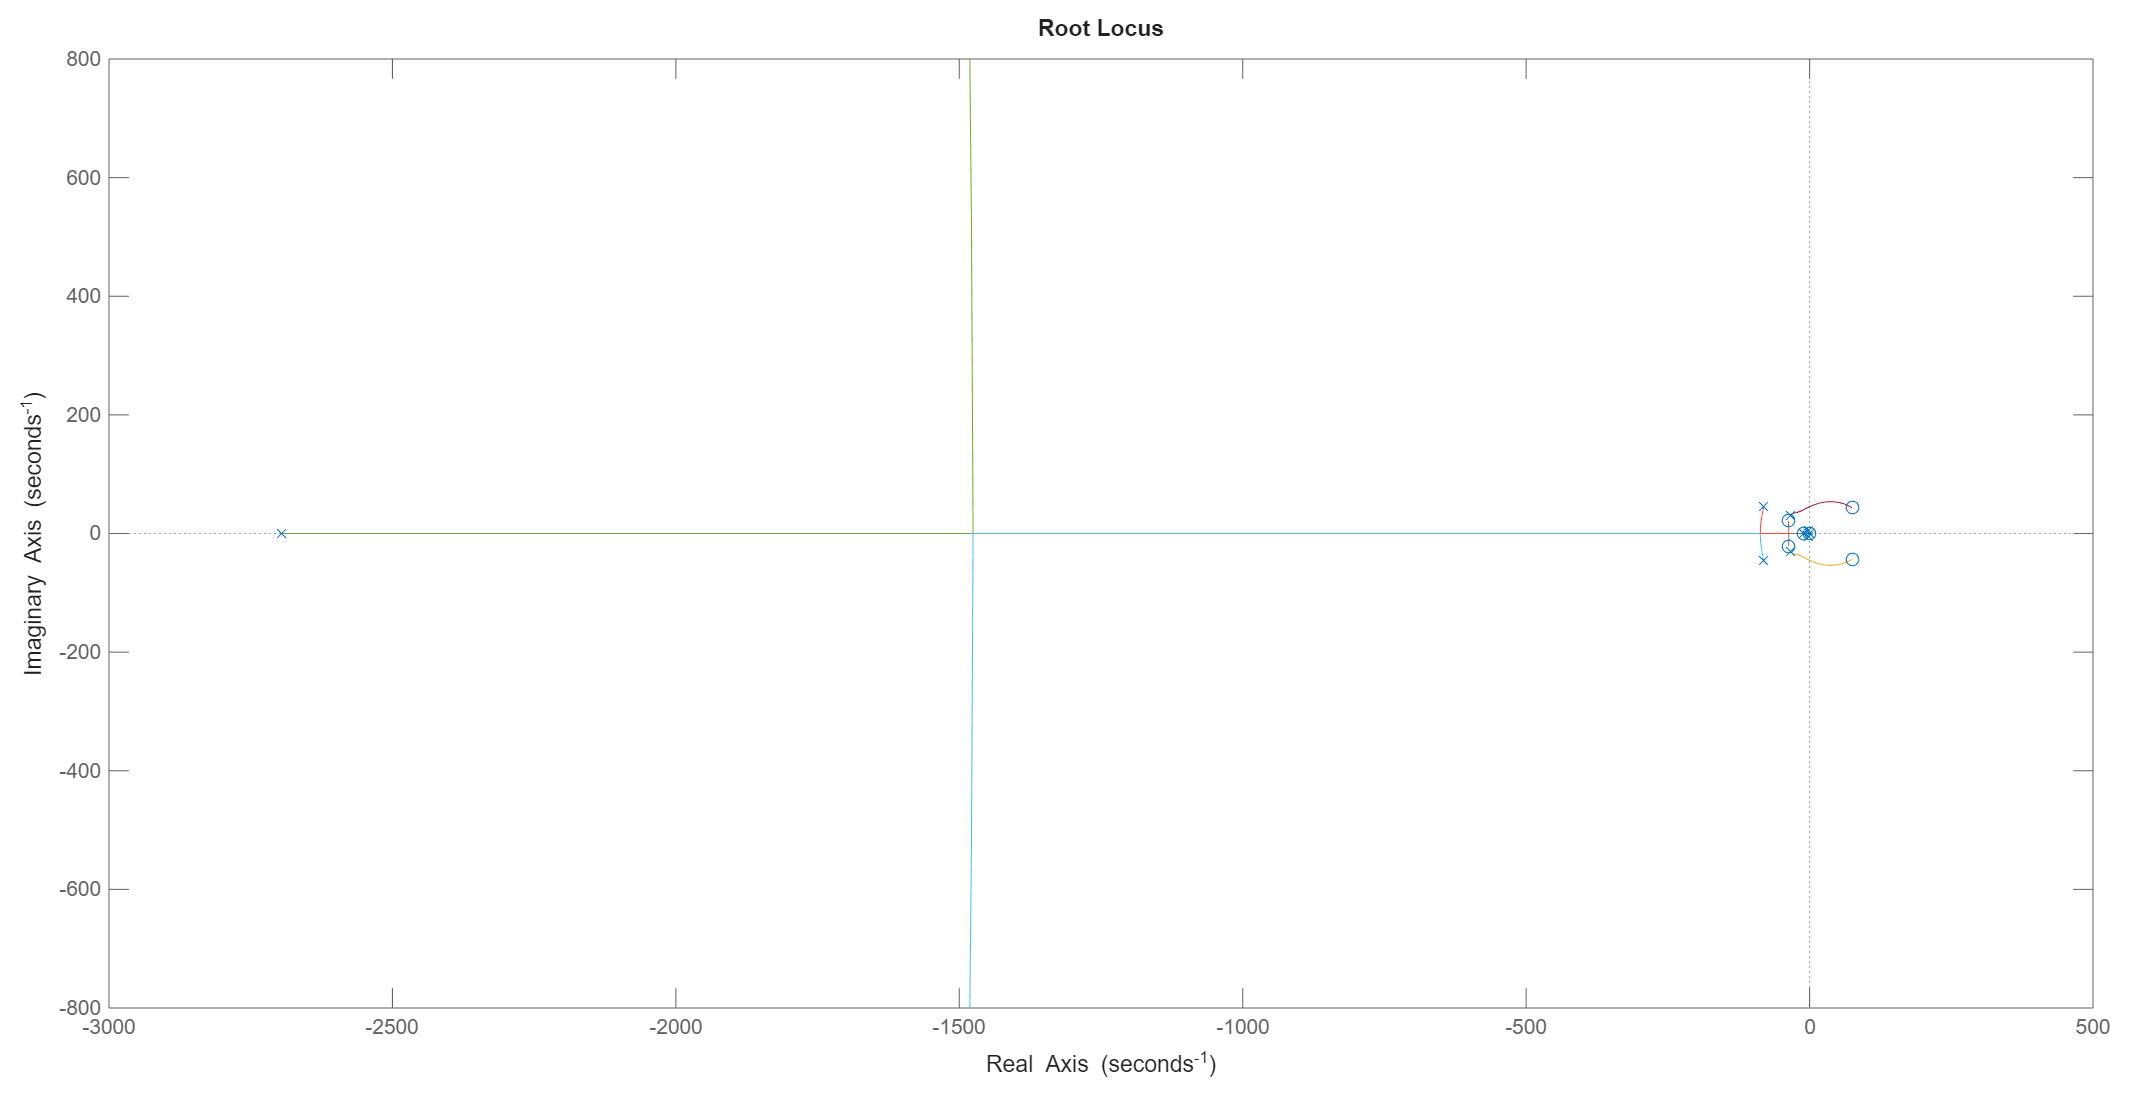
\includegraphics[scale = 0.45]{Cap3/rlocuscontroladoel.eps}
	\caption{Root locus plot for Elevation Axis.}\label{rlocus_el}
\end{figure}

Similarly, the root locus plot for the azimuth axis (Figure \ref{rlocus_az}) offers insights into its dynamic behavior. Given the simplifications made in the gimbal model, which often lead to analogous dynamics for both axes, one might anticipate similar characteristics to the elevation axis. However, subtle differences in inertia, friction, or controller parameters could result in distinct behaviors. By analyzing this plot, we can conclude that the poles of elevation axis system are in the left plane, meaning the system is stable.

\begin{figure}[H]
	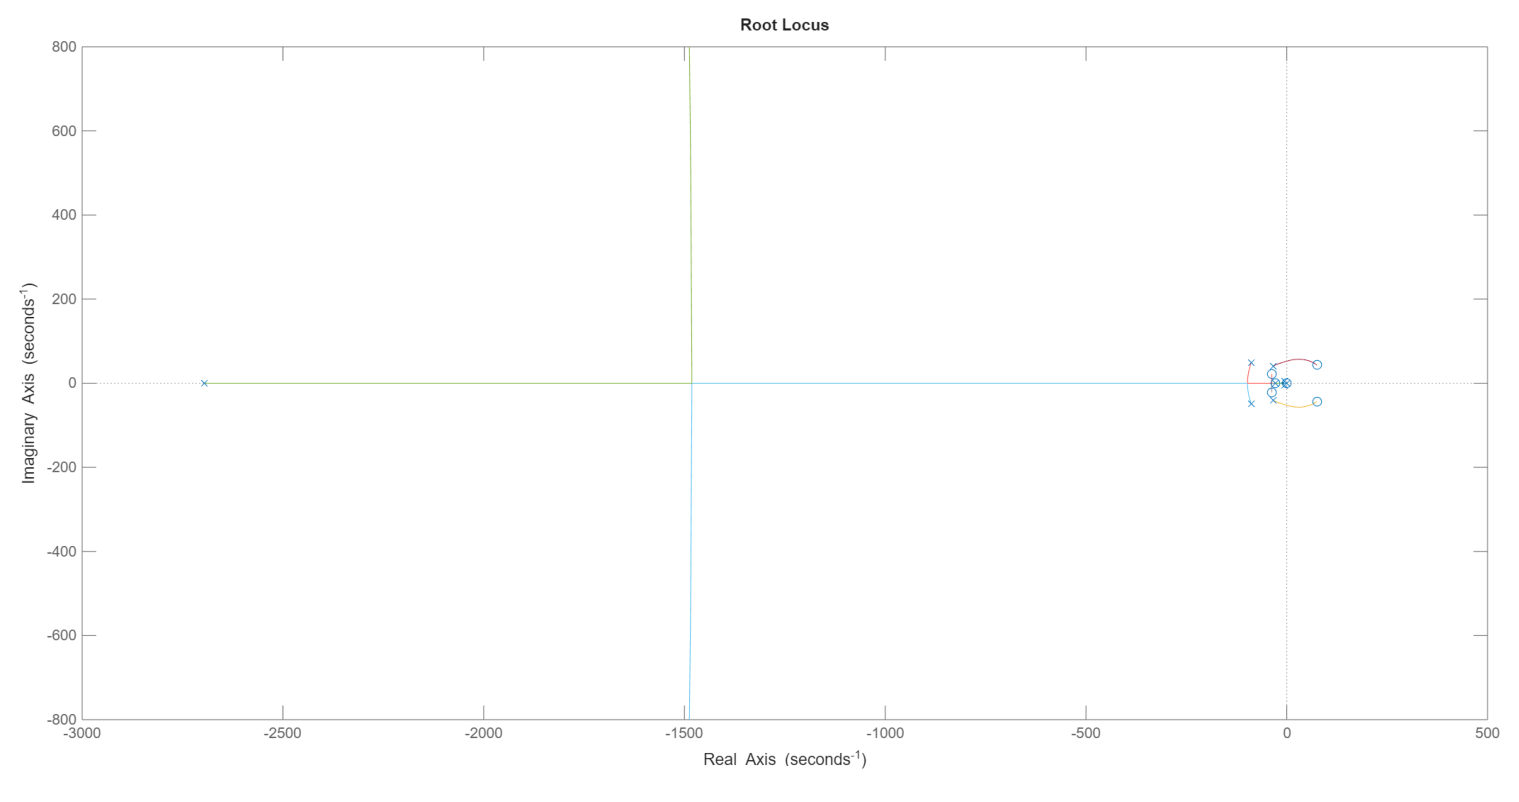
\includegraphics[scale = 0.6]{Cap3/rlocuscontroladoaz.eps}
	\caption{Root locus plot for Azimuth Axis.}\label{rlocus_az}
\end{figure}

The rlocus() function in MATLAB is particularly useful in the design of PID controllers. Analyzing the root locus plots provides a deeper understanding of why certain gains are effective and how they influence the closed-loop pole locations. For instance, the addition of an integral term introduces a pole at the origin, which helps eliminate steady-state error but can push the locus towards instability, often requiring a compensating zero. Conversely, a derivative term introduces a zero, pulling the root locus branches to the left, thereby improving stability and speeding up the transient response. By visualizing these effects on the root locus, it becomes possible to strategically place controller poles and zeros, and then adjust the overall gain to position the closed-loop poles in desired regions of the $s$-plane, ultimately achieving the specified performance criteria for both the elevation and azimuth axes of the gimbal.

After obtaining the initial gains via root locus, a fine-tuning process was employed. This fine-tuning involved using the \texttt{pidtune()} function associated with repeatedly simulating the closed-loop system and observing its response to different input scenarios. Small iterative modifications to the values of $K_p$, $K_i$, and $K_d$ were made to optimize the controller's performance regarding desired specifications, such as settling time, overshoot, and absence of steady-state error, ensuring that the system responded effectively and stably to the demands of object tracking. The final parameters for the PID in each axis are expressed in Table \ref{PID parameters table}.
\begin{table}[H]
\begin{center}
\caption{PID controller parameters for each axis.}
\label{PID parameters table}
\begin{tabular}{|c||c|||c|} 
 \hline
 Parameter & Elevation axis & Azimuth axis \\ [0.5ex] 
 \hline\hline
 $K_p$ & 0.5 & 0.5\\ 
 \hline
 $K_i$ & 0.15 & 0.2\\
 \hline
 $K_d$ & 0.5 & 0.45\\
 \hline
\end{tabular}
\end{center}
\end{table}
Figure \ref{PIDcontroleraxis} shows the controller for the elevation axis. The azimuth axis followed the same principle of implementation.
\begin{figure}[H]
	\centering
	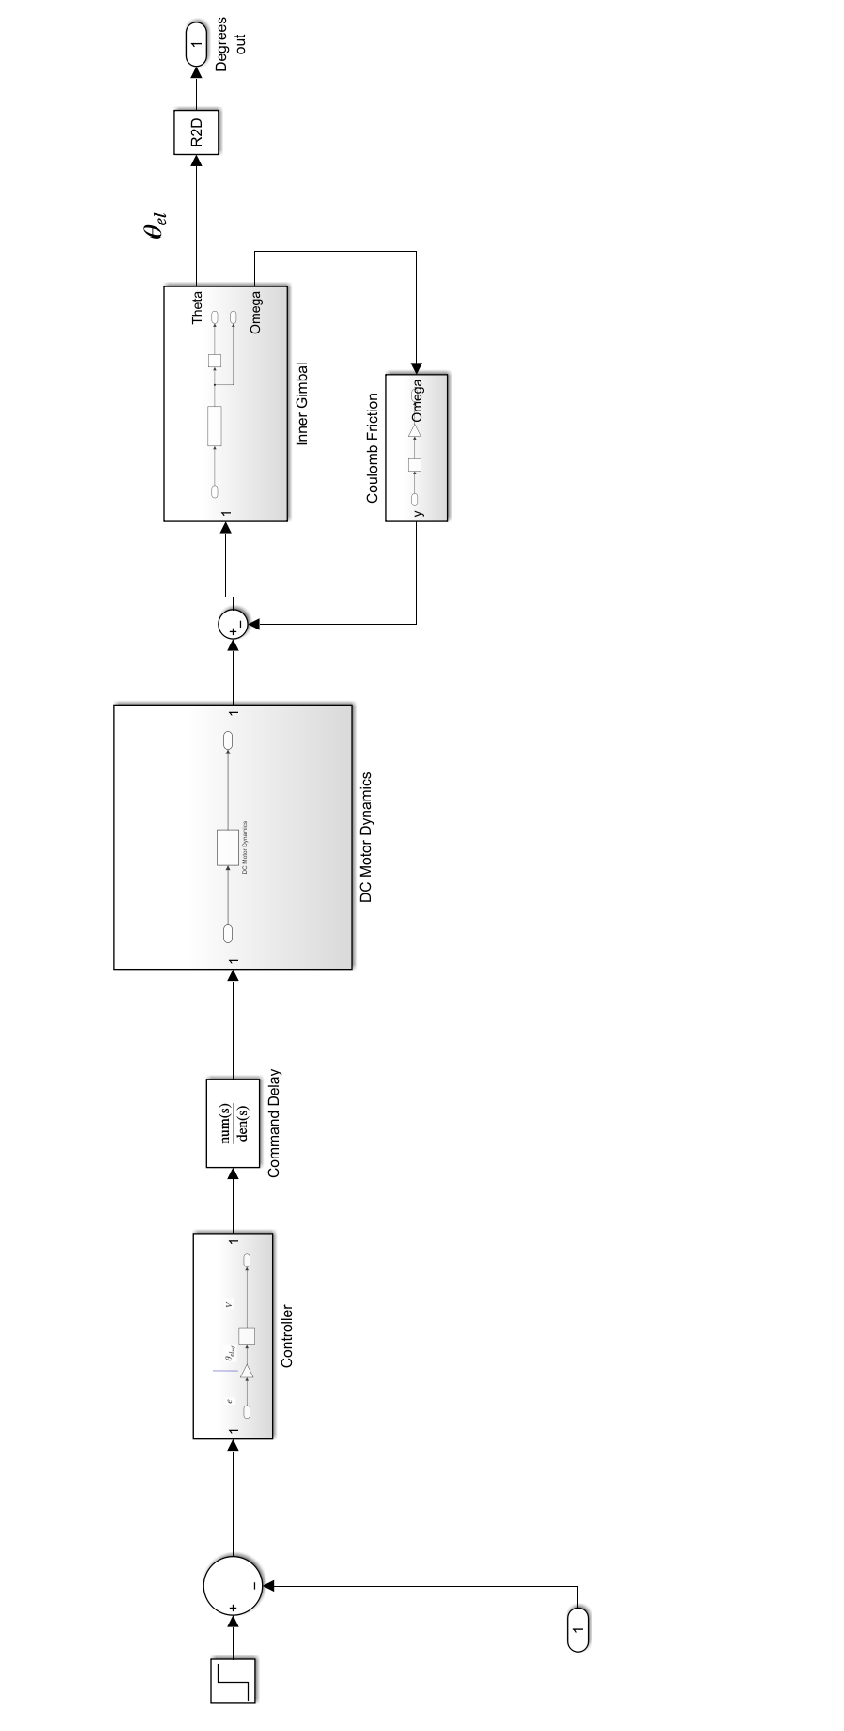
\includegraphics[scale = 0.85]{Cap3/PIDelevation.eps}
	\caption{PID controller implemented in Elevation Axis.}\label{PIDcontroleraxis}
\end{figure}
